% --------------------------------------------------------------------
% LaTeX Template for Math Worksheets
% --------------------------------------------------------------------
\documentclass{article}

% --- PACKAGE IMPORTS ---
% These packages add functionality for math symbols, formatting, etc.
\usepackage[margin=.7in]{geometry}       % For setting page margins to 0.7 inch
\usepackage{amsmath, amssymb, amsthm}   % American Mathematical Society packages for advanced math
\usepackage{graphicx}                   % For including images
\usepackage{fancyhdr}                   % For creating custom headers and footers
\usepackage[colorlinks=true, urlcolor=blue, linkcolor=blue]{hyperref} % For clickable links
\usepackage{cancel}
\usepackage{array}
\usepackage{amsfonts}
\usepackage{amsxtra}
\usepackage{epsfig}
\usepackage{wasysym}
\usepackage{relsize}
\usepackage{tikz}
\tikzset{every picture/.style={scale=1.2}}
\renewcommand{\normalsize}{\fontsize{12}{20}\selectfont}

% custom commands
\newcommand{\myauthor}{Miguel Gomez}
\newcommand{\canceling}[2]{\textcolor{red}{\cancelto{\textcolor{black}{#1}}{\textcolor{black}{#2}}}}
\newcommand{\todo}[1]{\textcolor{blue}{TODO:#1}}

% --- DOCUMENT & AUTHOR INFORMATION ---
\title{Worksheet \# 3}
\author{
  MATH 3160 -- Complex Variables\\
  \myauthor
}
\date{Completed: \today} 

% --- HEADER & FOOTER CONFIGURATION ---
% This section sets up the header that will appear on each page.
\pagestyle{fancy}
\fancyhf{} % Clears the default header and footer
\lhead{Math 3160 -- Worksheet \# 3} % Left side of header
\rhead{\myauthor} % Puts the author's name on the right side
\rfoot{Page \thepage} % Puts the page number on the bottom right

\begin{document}

\maketitle % This command generates the title based on the information above.

% ====================================================================
% --- START OF PROBLEMS ---
% ====================================================================

% Note: \section* creates a section heading without a number.
\section*{Problem 1}
Show that Re$(z) = \frac{z+\bar z}{2}$ and Im$(z)\cdot i = \frac{z-\bar z}{2}$ for any complex number $z = a+bi$:

Expressing the two as complex numbers and reducing:
\begin{align*}
\text{Re}(z) &= \frac{z+\bar z}{2} = \frac{a+bi+a-bi}{2} = \frac{2a}{2} = a = \text{Re}(z) \\
\text{Im}(z)\cdot i &= \frac{z-\bar z}{2} = \frac{a+bi-a+bi}{2} = \frac{2bi}{2} = bi = \text{Im}(z)\cdot i \\
\end{align*}

\hrule % Adds a horizontal line to separate problems.

\newpage
\section*{Problem 2}
Find the fourth roots of $-8-8\sqrt{3}i$. express the roots in rectangular coordinates, exhibit them as the vertices of a certain square, and point out the principal root.

\begin{align*}
  -8 -8\sqrt{3}i &= -8(1+\sqrt{3}) = 16(-1)\left(\frac{1+\sqrt{3}}{2}\right) =\\
  16e^{i\pi}e^{\frac{\pi}{3}} &= 16e^{i\frac{3\pi}{3}}e^{\frac{\pi}{3}} = 16e^{i\frac{4\pi}{3}} = 16e^{i\frac{-2\pi}{3}} \\
  16 &= 2^4 \\
  16e^{i\frac{-2\pi}{3}} = 2^4e^{i\frac{-2\pi}{3}}
\end{align*}
Starting from this point, we can take the $4^{\text{th}}$ root and then rotate that root by $\frac{2\pi}{4} = \frac{\pi}{2}$ to find the rest of the points.
\begin{align*}
  (e^{i\frac{-2\pi}{3}})^{\frac{1}{4}} &= e^{i\frac{-2\pi}{12}}= e^{i\frac{-\pi}{6}}\\
  e^{i(\frac{-\pi}{6} + \frac{3\pi}{6})} &= e^{i\frac{2\pi}{6}} = e^{i\frac{\pi}{3}}\\
  e^{i\frac{2\pi+3\pi}{6}} &= e^{i\frac{5\pi}{6}} \\
  e^{i\frac{5+3\pi}{6}} &= e^{i\left(\pi + \frac{2\pi}{6}\right)} = e^{i\left(\pi + \frac{\pi}{3}\right)} 
\end{align*}

So the principal root is the first root we get when moving counter-clockwise from 0, we get
\begin{align*}
  &= 2e^{i\frac{\pi}{3}}
\end{align*}
\begin{center}
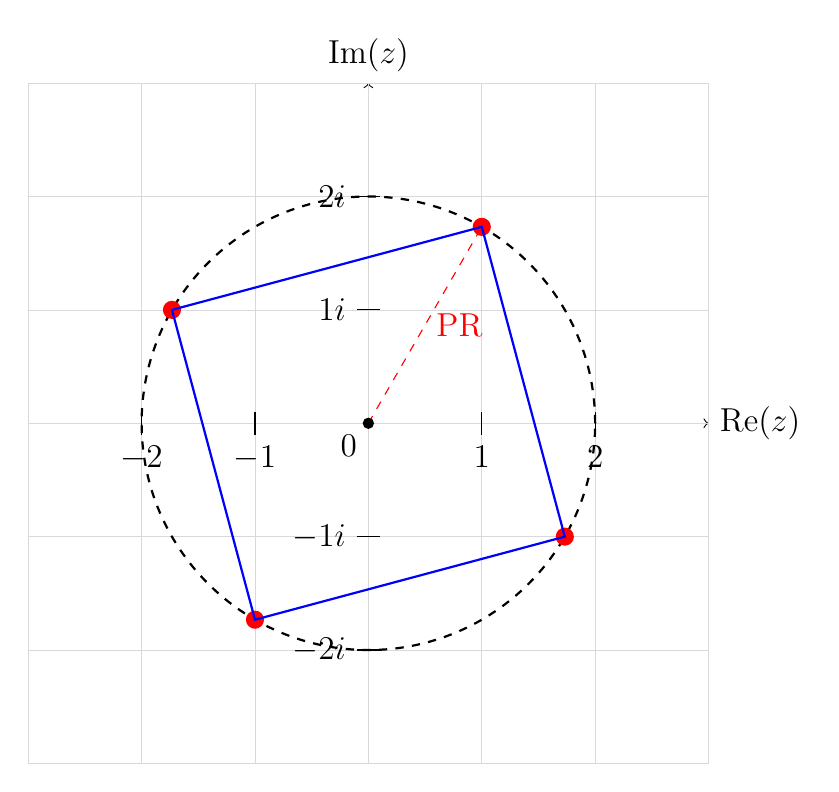
\begin{tikzpicture}[scale=1.2]
    % Draw axes
    \draw[->] (-3,0) -- (3,0) node[right] {$\text{Re}(z)$};
    \draw[->] (0,-3) -- (0,3) node[above] {$\text{Im}(z)$};
    
    % Add grid for better visualization
    \draw[gray!30, very thin] (-3,-3) grid (3,3);
    
    % Mark axis labels
    \foreach \x in {-2, -1, 1,2} {
        \draw (\x,0.1) -- (\x,-0.1) node[below] {$\x$};
    }
    \foreach \y in {-2,-1,1, 2} {
        \draw (0.1,\y) -- (-0.1,\y) node[left] {$\y i$};
    }
    
    % Define coordinates (fix the syntax)
    \coordinate (nthrootA) at (1.73205,-1);
    \coordinate (nthrootB) at (1,1.73205);
    \coordinate (nthrootC) at (-1.73205,1);
    \coordinate (nthrootD) at (-1,-1.73205);
    
    % Draw circle of radius 2 (black dashed)
    \draw[black, dashed, thick] (0,0) circle (2);
    
    % Mark the nth root points in red
    \fill[red] (nthrootA) circle (0.08);
    \fill[red] (nthrootB) circle (0.08);
    \draw[red, dashed] (0,0) -- (nthrootB) node[midway, above, right] {PR};
    \fill[red] (nthrootC) circle (0.08);
    \fill[red] (nthrootD) circle (0.08);
    
    % Draw lines connecting roots to form square
    \draw[blue, thick] (nthrootA) -- (nthrootB) -- (nthrootC) -- (nthrootD) -- cycle;
    
    % Mark origin
    \fill[black] (0,0) circle (0.05);
    \node[below left] at (0,0) {$0$};
\end{tikzpicture}
\end{center}
\hrule

\newpage
\section*{Problem 3}
Find the four zeros of the polynomial $z^4+4$, given that one of them is:

\begin{align*}
  z_0 &= \sqrt{2}e^{i\frac{\pi}{4}} = 1+i
\end{align*}

Use these zeros to factor $z^4+4$ into quadratic factors with real coefficients.

The zeros would be equally spaced because the polynomial can be factored into four roots.
\begin{align*}
  z^4+4 &= (z^2)^2--4 = (z^2)^2-(2i)^2 = \\
  &(z^2 - 2i)(z^2 + 2i) \\
        &\text{First root can also be put in terms of a difference of squares}\\
  (z^2 - 2i) &= (z^2 - (\sqrt{2i})^2) = (z - \sqrt{2i})(z + \sqrt{2i})\\
        &\text{Second root can also be put in terms of a difference of squares}\\
  (z^2 + 2i) & = (z^2 -- 2i) = (z^2 -(\sqrt{2i}i)^2) = (z - \sqrt{2i}i)(z + \sqrt{2i}i)\\
        &= (z - \sqrt{2i})(z + \sqrt{2i})(z - \sqrt{2i}i)(z + \sqrt{2i}i)\\
        &\text{square root of i:}\\
  \sqrt{i} &= i^{\frac{1}{2}} = (e^{i\frac{\pi}{2}})^{\frac{1}{2}} = e^{i\frac{\pi}{4}}\\
        &\text{magnitude of zero is }\sqrt{2}
\end{align*}

$\therefore \text{The four zeros are the points at }\sqrt{2}\text{ from the center.}$ These all have angles that are $\pm 45^{\circ}$ from $0\ \text{and }\pi$.

\begin{center}
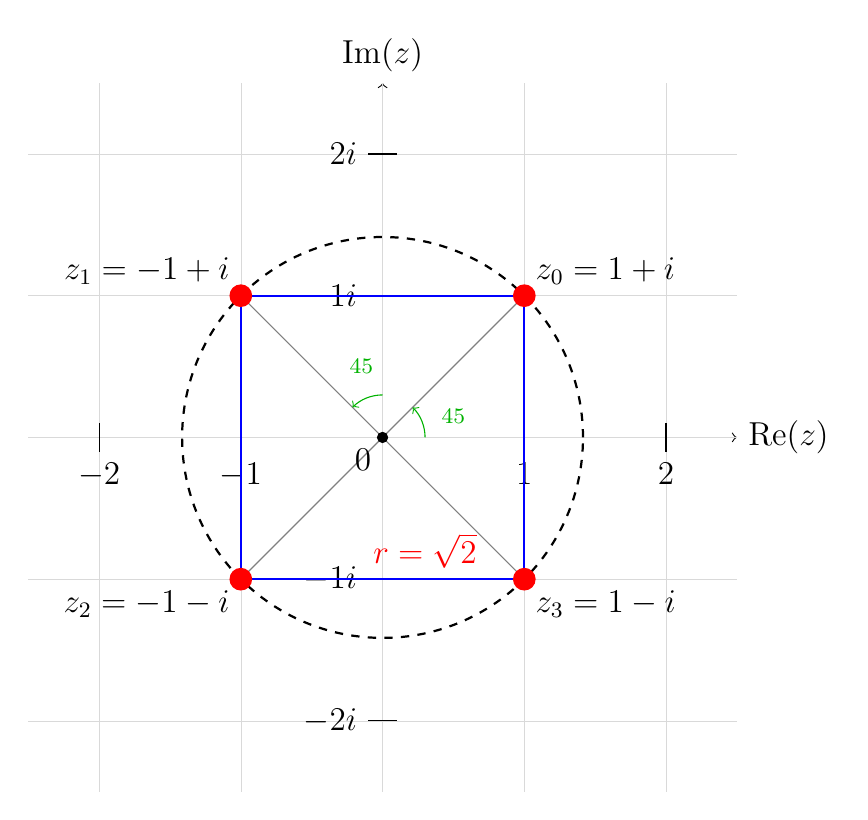
\begin{tikzpicture}[scale=1.5]
    % Draw axes
    \draw[->] (-2.5,0) -- (2.5,0) node[right] {$\text{Re}(z)$};
    \draw[->] (0,-2.5) -- (0,2.5) node[above] {$\text{Im}(z)$};
    
    % Add grid for better visualization
    \draw[gray!30, very thin] (-2.5,-2.5) grid (2.5,2.5);
    
    % Mark axis labels
    \foreach \x in {-2, -1, 1, 2} {
        \draw (\x,0.1) -- (\x,-0.1) node[below] {$\x$};
    }
    \foreach \y in {-2, -1, 1, 2} {
        \draw (0.1,\y) -- (-0.1,\y) node[left] {$\y i$};
    }
    
    % Define the four zeros (at distance √2 from origin)
    \coordinate (z0) at (1,1);      % √2 e^(iπ/4) = 1+i
    \coordinate (z1) at (-1,1);     % √2 e^(i3π/4) = -1+i  
    \coordinate (z2) at (-1,-1);    % √2 e^(i5π/4) = -1-i
    \coordinate (z3) at (1,-1);     % √2 e^(i7π/4) = 1-i
    
    % Draw circle of radius √2 (dashed)
    \draw[black, dashed, thick] (0,0) circle ({sqrt(2)});
    
    % Draw lines from origin to each zero (to show angles)
    \draw[gray, thin] (0,0) -- (z0);
    \draw[gray, thin] (0,0) -- (z1);
    \draw[gray, thin] (0,0) -- (z2);
    \draw[gray, thin] (0,0) -- (z3);
    
    % Draw the square connecting the zeros
    \draw[blue, thick] (z0) -- (z1) -- (z2) -- (z3) -- cycle;
    
    % Mark the four zeros as red points
    \fill[red] (z0) circle (0.08);
    \fill[red] (z1) circle (0.08);
    \fill[red] (z2) circle (0.08);
    \fill[red] (z3) circle (0.08);
    
    % Label the zeros
    \node[above right] at (z0) {$z_0 = 1+i$};
    \node[above left] at (z1) {$z_1 = -1+i$};
    \node[below left] at (z2) {$z_2 = -1-i$};
    \node[below right] at (z3) {$z_3 = 1-i$};
    
    % Add angle measurements
    \draw[green!70!black, ->] (0.3,0) arc (0:45:0.3);
    \node[green!70!black] at (0.5,0.15) {\footnotesize $45°$};
    
    \draw[green!70!black, ->] (0,0.3) arc (90:135:0.3);
    \node[green!70!black] at (-0.15,0.5) {\footnotesize $45°$};
    
    % Mark origin
    \fill[black] (0,0) circle (0.04);
    \node[below left] at (0,0) {$0$};
    
    % Add radius label
    \node[red] at (0.3, -0.8) {$r = \sqrt{2}$};
    
\end{tikzpicture}
\end{center}
\vspace{1cm} % Space for work


\section*{Problem 4}
Sketch the following sets and state whether each set is open, connected, a domain, and whether it is bounded.
\begin{enumerate}
  \item[(a)] $|z - 2 + i| \le 1$
\begin{center}
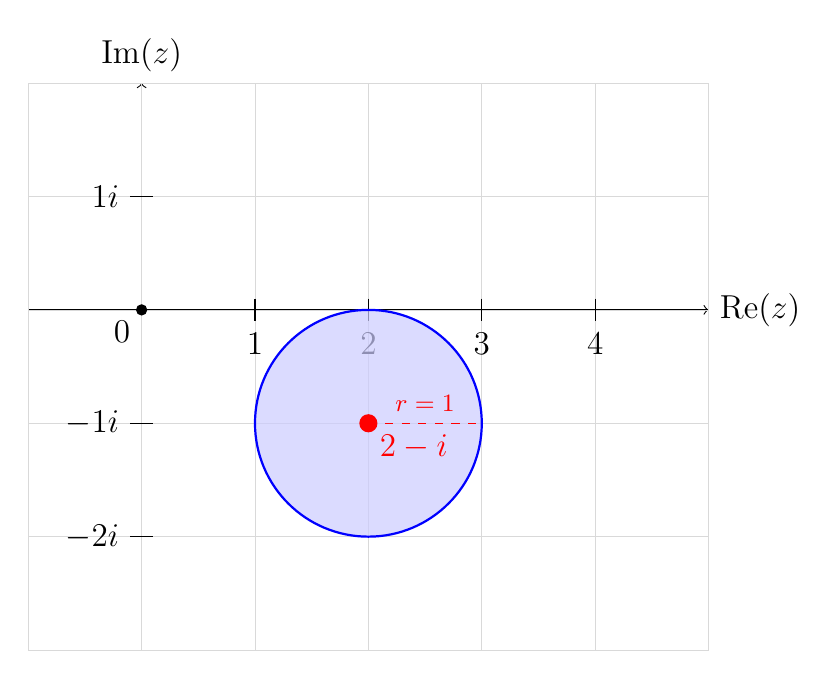
\begin{tikzpicture}[scale=1.2]
    % Draw axes
    \draw[->] (-1,0) -- (5,0) node[right] {$\text{Re}(z)$};
    \draw[->] (0,-3) -- (0,2) node[above] {$\text{Im}(z)$};
    
    % Add grid for better visualization
    \draw[gray!30, very thin] (-1,-3) grid (5,2);
    
    % Mark axis labels
    \foreach \x in {1,2,3,4} {
        \draw (\x,0.1) -- (\x,-0.1) node[below] {$\x$};
    }
    \foreach \y in {-2,-1,1} {
        \draw (0.1,\y) -- (-0.1,\y) node[left] {$\y i$};
    }
    
    % Define center and radius for |z - 2 + i| ≤ 1
    % Note: z - 2 + i = 0 means z = 2 - i, so center is at (2, -1)
    \def\centerx{2}
    \def\centery{-1}
    \def\radius{1}
    
    % Shade the region (closed disk)
    \fill[blue!20, opacity=0.7] (\centerx,\centery) circle (\radius);
    
    % Draw the boundary circle (solid line since it's ≤)
    \draw[thick, blue] (\centerx,\centery) circle (\radius);
    
    % Mark the center point
    \fill[red] (\centerx,\centery) circle (0.08);
    \node[red, below right] at (\centerx,\centery) {$2-i$};
    
    % Add radius indicator
    \draw[dashed, red] (\centerx,\centery) -- (\centerx+\radius,\centery);
    \node[red, above, font=\small] at (\centerx+\radius/2,\centery) {$r=1$};
    
    % Mark origin
    \fill[black] (0,0) circle (0.05);
    \node[below left] at (0,0) {$0$};
\end{tikzpicture}
\end{center}

\begin{itemize}
    \item \textbf{Open:} No, because the boundary is included ($\le$ condition)
    \item \textbf{Connected:} Yes, it's a disk which is connected
    \item \textbf{Domain:} No, because it's not open
    \item \textbf{Bounded:} Yes, all points are within distance 1 from center $(2,-1)$
\end{itemize}

\newpage
\item[(b)] $|2z+3| > 4$
\begin{center}
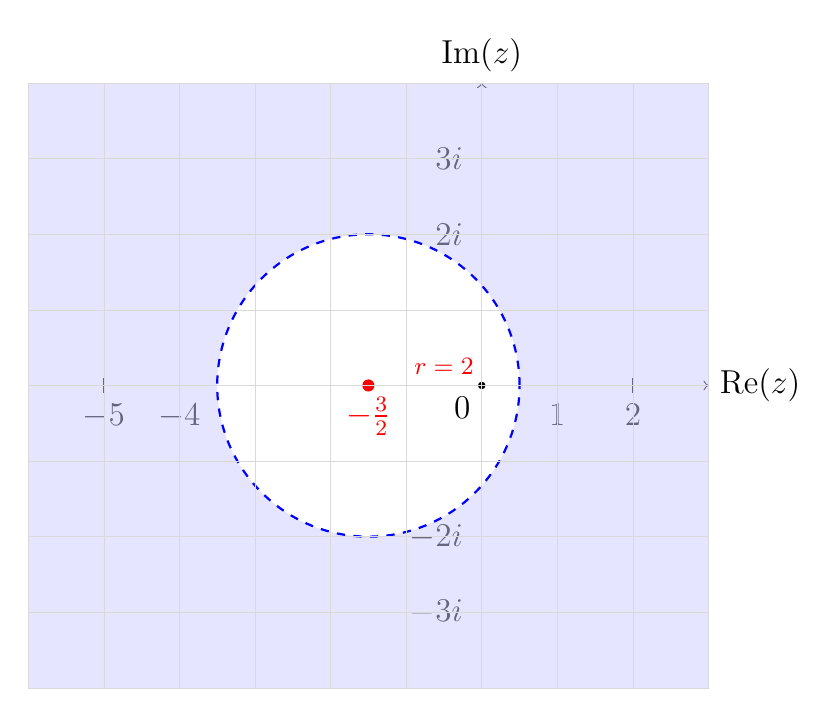
\begin{tikzpicture}[scale=0.8]
    % Draw axes
    \draw[->] (-6,0) -- (3,0) node[right] {$\text{Re}(z)$};
    \draw[->] (0,-4) -- (0,4) node[above] {$\text{Im}(z)$};
    
    % Mark axis labels
    \foreach \x in {-5,-4,-3,-2,-1,1,2} {
        \draw (\x,0.1) -- (\x,-0.1) node[below] {$\x$};
    }
    \foreach \y in {-3,-2,-1,1,2,3} {
        \draw (0.1,\y) -- (-0.1,\y) node[left] {$\y i$};
    }
    
    % |2z+3| > 4 means |z + 3/2| > 2
    % Center at (-3/2, 0), radius 2
    \def\centerx{-1.5}
    \def\centery{0}
    \def\radius{2}
    
    % Shade the exterior region
    \fill[blue!20, opacity=0.5] (-6,-4) rectangle (3,4);
    \fill[white] (\centerx,\centery) circle (\radius);
    
    % Draw the boundary circle (dashed since it's excluded)
    \draw[thick, blue, dashed] (\centerx,\centery) circle (\radius);
    
    % Mark the center point
    \fill[red] (\centerx,\centery) circle (0.08);
    \node[red, below] at (\centerx,\centery) {$-\frac{3}{2}$};
    
    % Add radius indicator
    \draw[dashed, red] (\centerx,\centery) -- (\centerx+\radius,\centery);
    \node[red, above, font=\small] at (\centerx+\radius/2,\centery) {$r=2$};
    
    % Mark origin
    \fill[black] (0,0) circle (0.05);
    \node[below left] at (0,0) {$0$};
        % Add grid
    \draw[gray!30, very thin] (-6,-4) grid (3,4);

\end{tikzpicture}
\end{center}
\begin{itemize}
    \item \textbf{Open:} Yes, because boundary is not included
    \item \textbf{Connected:} Yes because the region outside the disk is connected
    \item \textbf{Domain:} Yes, open and connected are satisfied
    \item \textbf{Bounded:} No, the region extends to infinity
\end{itemize}
\newpage
\item[(c)] Im$(z) > 1$
\begin{center}
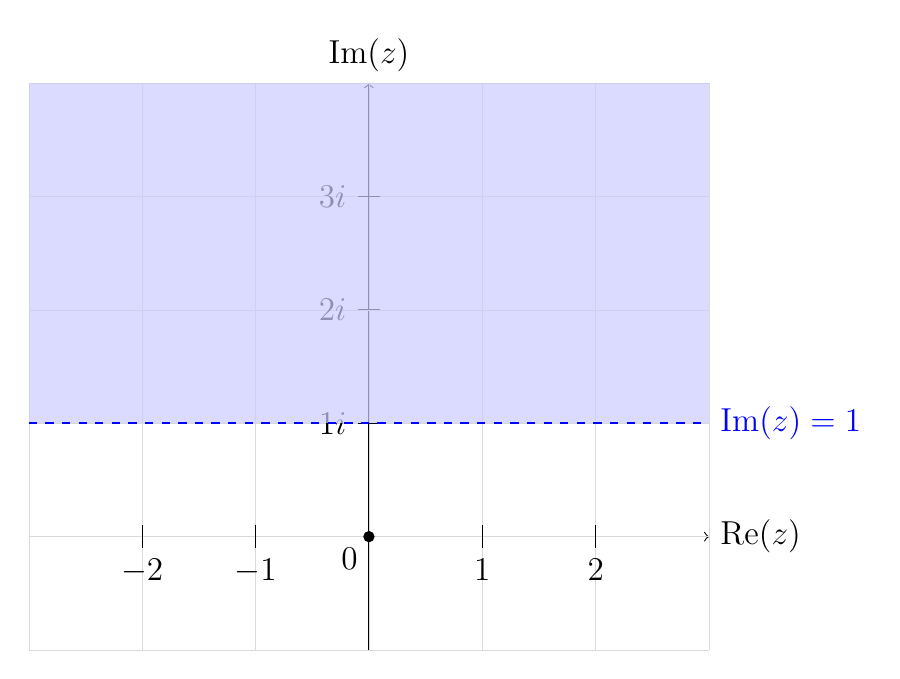
\begin{tikzpicture}[scale=1.2]
    % Draw axes
    \draw[->] (-3,0) -- (3,0) node[right] {$\text{Re}(z)$};
    \draw[->] (0,-1) -- (0,4) node[above] {$\text{Im}(z)$};
    
    % Add grid
    \draw[gray!30, very thin] (-3,-1) grid (3,4);
    
    % Mark axis labels
    \foreach \x in {-2,-1,1,2} {
        \draw (\x,0.1) -- (\x,-0.1) node[below] {$\x$};
    }
    \foreach \y in {1,2,3} {
        \draw (0.1,\y) -- (-0.1,\y) node[left] {$\y i$};
    }
    
    % Shade the region Im(z) > 1
    \fill[blue!20, opacity=0.7] (-3,1) rectangle (3,4);
    
    % Draw the boundary line Im(z) = 1 (dashed since excluded)
    \draw[thick, blue, dashed] (-3,1) -- (3,1);
    \node[blue, right] at (3,1) {$\text{Im}(z) = 1$};
    
    % Mark origin
    \fill[black] (0,0) circle (0.05);
    \node[below left] at (0,0) {$0$};
\end{tikzpicture}
\end{center}
\begin{itemize}
    \item \textbf{Open:} Yes, because boundary is not included
    \item \textbf{Connected:} Yes because the region above the line Im$(z) = 1$ is connected
    \item \textbf{Domain:} Yes, open and connected are satisfied
    \item \textbf{Bounded:} No, the region extends to infinity
\end{itemize}

\newpage
\item[(d)] Im$(z) = 1$
\begin{center}
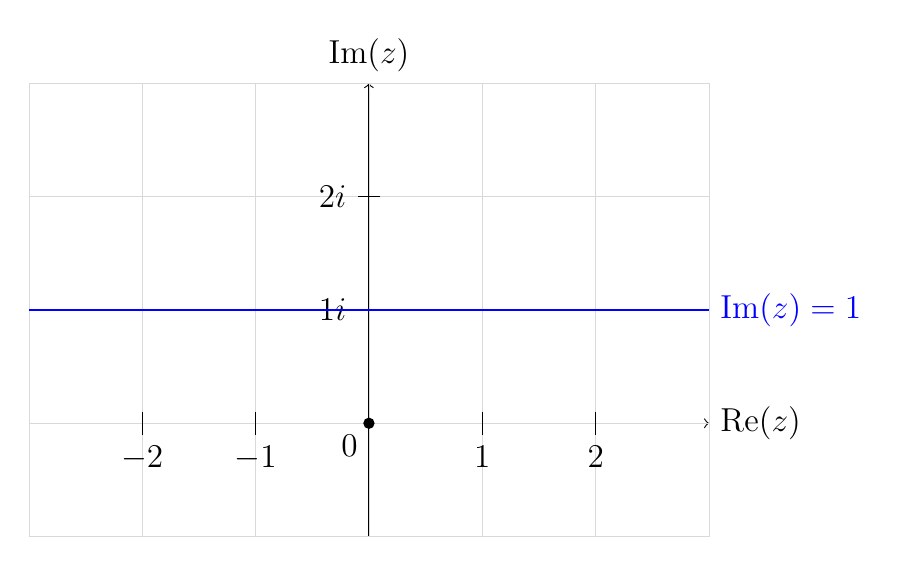
\begin{tikzpicture}[scale=1.2]
    % Draw axes
    \draw[->] (-3,0) -- (3,0) node[right] {$\text{Re}(z)$};
    \draw[->] (0,-1) -- (0,3) node[above] {$\text{Im}(z)$};
    
    % Add grid
    \draw[gray!30, very thin] (-3,-1) grid (3,3);
    
    % Mark axis labels
    \foreach \x in {-2,-1,1,2} {
        \draw (\x,0.1) -- (\x,-0.1) node[below] {$\x$};
    }
    \foreach \y in {1,2} {
        \draw (0.1,\y) -- (-0.1,\y) node[left] {$\y i$};
    }
    
    % Draw the line Im(z) = 1 (solid since it's the set)
    \draw[thick, blue] (-3,1) -- (3,1);
    \node[blue, right] at (3,1) {$\text{Im}(z) = 1$};
    
    % Mark origin
    \fill[black] (0,0) circle (0.05);
    \node[below left] at (0,0) {$0$};
\end{tikzpicture}
\end{center}
\begin{itemize}
    \item \textbf{Open:} No, because line is included
    \item \textbf{Connected:} No because no region of radius $r$ can be formed on a line
    \item \textbf{Domain:} No, open and connected aren't satisfied
    \item \textbf{Bounded:} No, the line extends to infinity and there is no region
\end{itemize}

\newpage
  \item[(e)] $0 \le \text{arg}(z) \le \frac{\pi}{4}$, where $z \neq 0$
\begin{center}
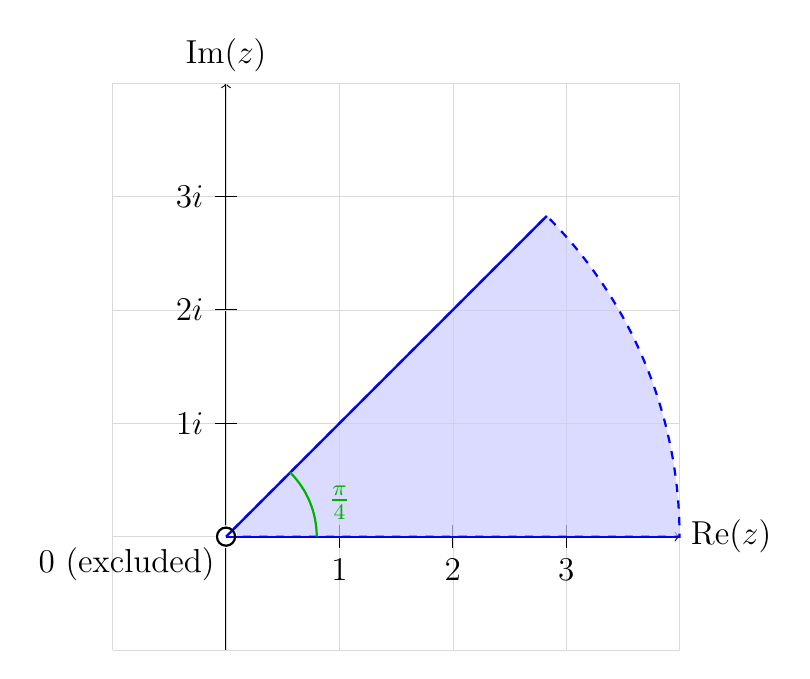
\begin{tikzpicture}[scale=1.2]
    % Draw axes
    \draw[->] (-1,0) -- (4,0) node[right] {$\text{Re}(z)$};
    \draw[->] (0,-1) -- (0,4) node[above] {$\text{Im}(z)$};
    
    % Add grid
    \draw[gray!30, very thin] (-1,-1) grid (4,4);
    
    % Mark axis labels
    \foreach \x in {1,2,3} {
        \draw (\x,0.1) -- (\x,-0.1) node[below] {$\x$};
    }
    \foreach \y in {1,2,3} {
        \draw (0.1,\y) -- (-0.1,\y) node[left] {$\y i$};
    }
    
    % Draw the sector from arg = 0 to arg = π/4
    \fill[blue!20, opacity=0.7] (0,0) -- (4,0) arc (0:45:4) -- cycle;
    % Draw the sector outline with dashed line
    \draw[blue, thick, dashed] (0,0) -- (4,0) arc (0:45:4) -- cycle;    
    % Remove the origin (small white circle)
    \fill[white] (0,0) circle (0.1);
    
    % Draw the boundary rays (solid since included)
    \draw[thick, blue] (0,0) -- (4,0);
    \draw[thick, blue] (0,0) -- ({4*cos(45)}, {4*sin(45)});
    
    % Add angle arc
    \draw[green!70!black, thick] (0.8,0) arc (0:45:0.8);
    \node[green!70!black] at (1,0.3) {$\frac{\pi}{4}$};
    
    % Mark origin (excluded)
    \draw[black, thick] (0,0) circle (0.08);
    \node[below left] at (0,0) {$0$ (excluded)};
\end{tikzpicture}
\end{center}

\begin{itemize}
    \item \textbf{Open:} No, because boundary is included
    \item \textbf{Connected:} Yes because the region inside the arc is connected
    \item \textbf{Domain:} No, because both open and connected aren't satisfied
    \item \textbf{Bounded:} No, the region within the arc extends to infinity
\end{itemize}

\newpage

\item[(f)] $|z - 4| \geq |z|$

  Equal at $z = 2$. If $z = 0$, then the expression holds. $4 \geq 0$. If $z > 2$, then we get a false condition. say it were $3$:
  \begin{align*}
    |3 - 4| \geq |3| &\xrightarrow{} |-1| \ngeq |3| 
  \end{align*}
  
  %Interestingly, I think this is simple to show by the meet of two circles. These are precicely equal when they meet at $z = 2$
  \begin{center}
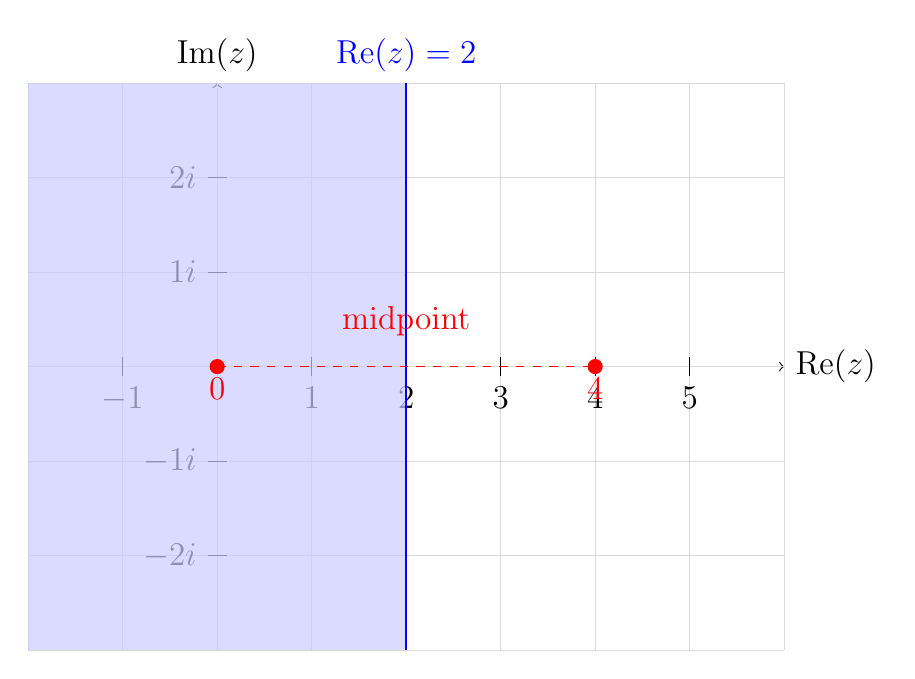
\begin{tikzpicture}[scale=1.0]
    % Draw axes
    \draw[->] (-2,0) -- (6,0) node[right] {$\text{Re}(z)$};
    \draw[->] (0,-3) -- (0,3) node[above] {$\text{Im}(z)$};
    
    % Add grid
    \draw[gray!30, very thin] (-2,-3) grid (6,3);
    
    % Mark axis labels
    \foreach \x in {-1,1,2,3,4,5} {
        \draw (\x,0.1) -- (\x,-0.1) node[below] {$\x$};
    }
    \foreach \y in {-2,-1,1,2} {
        \draw (0.1,\y) -- (-0.1,\y) node[left] {$\y i$};
    }
    
    % Shade the region Re(z) ≤ 2 (left half-plane)
    \fill[blue!20, opacity=0.7] (-2,-3) rectangle (2,3);
    
    % Draw the boundary line x = 2 (solid since included)
    \draw[thick, blue] (2,-3) -- (2,3);
    \node[blue, above] at (2,3) {Re$(z) = 2$};
    
    % Mark the points 0 and 4
    \fill[red] (0,0) circle (0.08);
    \fill[red] (4,0) circle (0.08);
    \node[red, below] at (0,0) {$0$};
    \node[red, below] at (4,0) {$4$};
    
    % Draw dashed line showing the midpoint
    % \draw[black, dashed] (0,0) circle (2);
    % \draw[black, dashed] (4,0) circle (2);

    % \draw[black, dashed] (0,0) circle (2.5);
    % \draw[black, dashed] (4,0) circle (2.5);

    % \draw[black, dashed] (0,0) circle (3);
    % \draw[black, dashed] (4,0) circle (3);

    \draw[red, dashed] (0,0) -- (4,0);
    \node[red, above] at (2,0.2) {midpoint};
\end{tikzpicture}
\end{center}

\begin{itemize}
    \item \textbf{Open:} No because the boundary is included.
    \item \textbf{Connected:} Yes because the region less than midpoint is connected
    \item \textbf{Domain:} No, because both open and connected aren't satisfied
    \item \textbf{Bounded:} No, the region less than midpoint extends to infinity
\end{itemize}

\end{enumerate}
\vspace{1cm} % Space for work

\hrule

% Add more problems as needed...
% \newpage
% \section*{Problem 4: [Problem Title]}
% [Problem statement or work space goes here]
% \hrule

\end{document}

%%% Local Variables:
%%% mode: latex
%%% TeX-master: t
%%% End:
